\documentclass[11pt,a4paper]{scrartcl}
\typearea{12}
\usepackage{enumitem}
\usepackage{graphicx}
\usepackage{pstricks}
\usepackage{listings}

\usepackage{tikz}

\usepackage{pgf}
\usepackage[utf8]{inputenc}
\usetikzlibrary{arrows,automata}
\usetikzlibrary{positioning}
\usetikzlibrary{shapes.symbols,shapes.callouts,patterns}

\tikzset{
    intro/.style={
      rectangle,
           draw=black, very thick,
           inner sep=2pt,
           text centered,
           minimum width=2.5cm,
           minimum height=1cm,
           },
}


\tikzset{
    big-oh/.style={
      rectangle,
           draw=red, very thick,
           inner sep=2pt,
           text centered,
           minimum width=2.5cm,
           minimum height=1cm,
           },
}


\tikzset{
    sorting/.style={
      rectangle,
           draw=blue, very thick,
           inner sep=2pt,
           text centered,
           minimum width=2.5cm,
           minimum height=1cm,
           },
}


\tikzset{
    graph/.style={
      rectangle,
           draw=yellow, very thick,
           inner sep=2pt,
           text centered,
           minimum width=2.5cm,
           minimum height=1cm,
           },
}


\tikzset{
    data/.style={
      rectangle,
           draw=green, very thick,
           inner sep=2pt,
           text centered,
           minimum width=2.5cm,
           minimum height=1cm,
           },
}


\tikzset{
    science/.style={
      rectangle,
           draw=orange, very thick,
           inner sep=2pt,
           text centered,
           minimum width=2.5cm,
           minimum height=1cm,
           },
}



\tikzset{
    sciencefaded/.style={
      rectangle,
           draw=orange, thin,
           inner sep=2pt,
           text centered,
           minimum width=2.5cm,
           minimum height=1cm,
           },
}






\lstset{language=python}
\pagestyle{headings}
\markright{Algorithms - course plan}

\begin{document}
\section*{Course plan}
\begin{center}
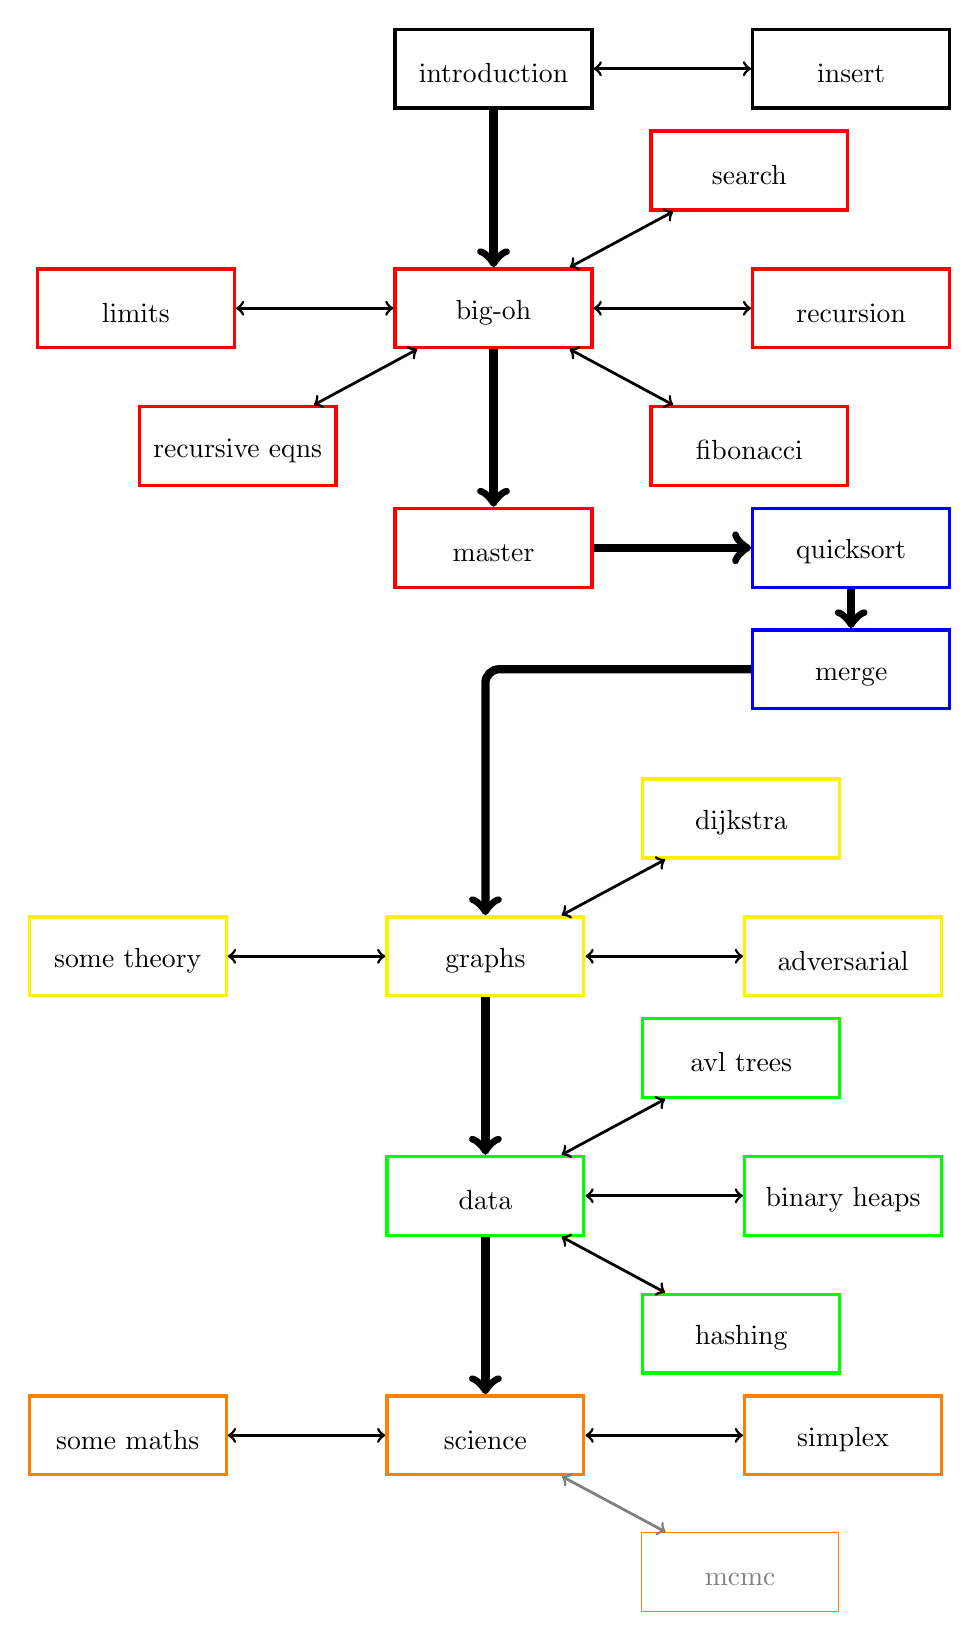
\begin{tikzpicture}

%post/.style={->,shorten >=2pt,>=stealth',semithick}

\node[intro,text height=0.35cm](int){introduction};
\node[intro,text height=0.35cm,right = 2cm of int](bse){insert};

\path (int) edge[<->,line width=1pt](bse);

\node[big-oh,text height=0.35cm,below = 2cm of int](boh){big-oh};
\node[big-oh,text height=0.35cm,left = 2cm of boh](lim){limits};
\node[big-oh,text height=0.35cm,below left = 1cm of boh](rma){recursive eqns};

\path (int) edge[->,line width=3pt](boh);
\path (boh) edge[<->,line width=1pt](rma);

\node[big-oh,text height=0.35cm,above right = 1cm of boh](sea){search};
\node[big-oh,text height=0.35cm,right = 2cm of boh](rec){recursion};
\node[big-oh,text height=0.35cm,below right = 1cm of boh](fib){fibonacci};

\path (boh) edge[<->,line width=1pt](lim);

\path (boh) edge[<->,line width=1pt](sea);
\path (boh) edge[<->,line width=1pt](rec);
\path (boh) edge[<->,line width=1pt](fib);

\node[big-oh,text height=0.35cm,below = 2cm of boh](mas){master};

\path (boh) edge[->,line width=3pt](mas);

\node[sorting,text height=0.35cm, right = 2cm of mas](qso){quicksort};
\node[sorting,text height=0.35cm,below = 0.5cm of qso](mso){merge};
%\node[sorting,text height=0.35cm,below = 0.5cm of mso](rso){radix};

\path (mas) edge[->,line width=3pt](qso);
\path (qso) edge[->,line width=3pt](mso);
%\path (mso) edge[->,line width=3pt](rso);

\node[left = 3.25cm of mso](null){};


\node[graph,text height=0.35cm,below = 3cm of null](gra){graphs};
\node[graph,text height=0.35cm,left = 2cm of gra](sth){some theory};

\draw[->,rounded corners=5pt,line width=3pt] (mso)-|(gra);


\node[graph,text height=0.35cm,above right = 1cm of gra](dij){dijkstra};
\node[graph,text height=0.35cm,right = 2cm of gra](ase){adversarial};

\path (gra) edge[<->,line width=1pt](dij);
\path (gra) edge[<->,line width=1pt](ase);
\path (gra) edge[<->,line width=1pt](sth);

\node[data,text height=0.35cm,below = 2cm of gra](btr){data};

\node[data,text height=0.35cm,above right = 1cm of btr](atr){avl trees};
\node[data,text height=0.35cm, right = 2cm of btr](bhe){binary heaps};
\node[data,text height=0.35cm,below right = 1cm of btr](has){hashing};

\path (gra) edge[->,line width=3pt](btr);
\path (btr) edge[<->,line width=1pt](atr);
\path (btr) edge[<->,line width=1pt](bhe);
\path (btr) edge[<->,line width=1pt](has);

\node[science,text height=0.35cm,below = 2cm of btr](sci){science};

\node[science,text height=0.35cm,left = 2cm of sci](sma){some maths};

\node[science,text height=0.35cm,right = 2cm of sci](sim){simplex};

\node[sciencefaded,text height=0.35cm,below right = 1cm of sci](mcmc){\textcolor{gray}{mcmc}};


\path (btr) edge[->,line width=3pt](sci);
\path (sci) edge[<->,line width=1pt](sim);
\path (sci) edge[<->,line width=1pt](sma);
\path (sci) edge[<->,line width=1pt,color=gray](mcmc);


\end{tikzpicture}
\end{center}

\section*{Key to the plan}

The nodes don't represent equal amounts of time, for example, the
fibonacci sequence node represents about half a lecture, whereas the
big-oh node might be two lectures.

\subsection*{Positions and colors}
\begin{itemize}
\item CENTRE: main topics
\item LEFT: background theory
\item RIGHT: examples and applications
\item \textcolor{red}{RED:} algorithmic complexity
\item \textcolor{blue}{BLUE:} sorting
\item \textcolor{yellow}{YELLOW:} graph theory
\item \textcolor{green}{GREEN:} data structures
\item \textcolor{orange}{ORANGE:} scientific computing
\end{itemize} 

\subsection*{Nodes}

\begin{enumerate}[label=(\alph*)]
\item \textbf{introduction:} What is an algorithm.
\item \textbf{insert:} Insert sort, an example algorithm.
\item \textbf{\textcolor{red}{big-oh}} Algorithmic complexity.
\item \textbf{\textcolor{red}{limits}} Limits in the mathematical sense.
\item \textbf{\textcolor{red}{recursive eqns}} How to solve recursive equations
\item \textbf{\textcolor{red}{search:}} Big-oh for binart and linear.
\item \textbf{\textcolor{red}{recursion:}} Recursion and recursive algorithms.
\item \textbf{\textcolor{red}{fibonacci:}} The interesting example of the fibonacci sequence. 
\item \textbf{\textcolor{red}{master:}} The master theorem.
\item \textbf{\textcolor{blue}{quicksort:}} Quicksort.
\item \textbf{\textcolor{blue}{merge sort:}} Merge sort.
%\item \textbf{\textcolor{blue}{radix sort:}} Radix sort.
\item \textbf{\textcolor{yellow}{graphs:}} Introduction to graph theory.
\item \textbf{\textcolor{yellow}{some theory:}} Some definitions and the Euler theorem. 
\item \textbf{\textcolor{yellow}{dikstra:}} Dijkskra's algorithm.
\item \textbf{\textcolor{yellow}{adversarial:}} Adversarial search algorithms.
\item \textbf{\textcolor{green}{data:}} Data structures, linked lists and binary trees.
\item \textbf{\textcolor{green}{avl trees:}} Balanced trees and the AVL rotations. 
\item \textbf{\textcolor{green}{binary heap:}} Binary heaps. 
\item \textbf{\textcolor{green}{hashing:}} Hash functions and hashing data. 
\item \textbf{\textcolor{orange}{science:}} Scientific computing.
\item \textbf{\textcolor{orange}{some math:}} Revising a bit of calculus.
\item \textbf{\textcolor{orange}{simplex:}} The Nelder Meade algorithm.
\item \textbf{\textcolor{orange}{mcmc:}} Markov chain Monte Carlo

\end{enumerate}

The last section is aspirational, it is likely there will not be time to discuss them and they will not be examined.

\end{document}

